\section{Comparative Anatomy of the Descending Pathways}

It must have felt uncanny to those early researchers to find that surface stimulation of the cortex produces discrete muscle responses, in a way so similar to what Galvani did with the frog's leg. Indeed, Sherrington himself conveys the feeling clearly in the opening of his seminal lecture on the motor cortex \cite[p.271]{Sherrington1906}, confessing ``that although it is not surprising that such territorial subdivision of function should exist in the cerebral cortex, it is surprising that by our relatively imperfect artifices for stimulation we should be able to obtain clear evidence thereof.''

Of course, it did not go unnoticed that this fact might be due to the massive projection from cortex to the spinal cord, which had been fully traced by Türck only twenty years before Fritsch and Hitzig's experiment \cite{Nathan1955}. This so-called ``pyramidal'' tract\footnote{The name ``pyramidal'' is derived from the fact that the tract passes through the medullary pyramids, a pair of white matter structures in the brainstem with a roughly pyramidal shape.} was found to originate in the anterior regions of the cerebral cortex and terminate directly in the lateral columns of the spinal cord after decussating (i.e. crossing over) at the level of the brainstem's \emph{medulla oblongata}. The presence of this corticospinal tract presented compelling visual evidence of the means by which the motor cortex might be able to exert such a direct influence on movement by electrical conduction of nerve impulses, but the underlying biological mechanism remained elusive.

\subsection{A Functional Theory for the Motor Cortex}

Only four years after the discovery of the motor cortex, the Ukrainian anatomist and histologist Vladimir Betz connected for the first time the macroscopic cerebral organization and function proposed by Hitzig and Ferrier with unique, detailed histological evidence of cells found in the motor region, in his remarkably insightful 1874 publication:

\blockquote[{\protect\cite{Betz1874, Kushchayev2012}}]{Such consistency in the region where these cells can be found, manifested as a very definitive cortical layer, as well as in a specific cerebral convolution, prompted me to devote my attention to that particular part of the animal brain, mainly the dog’s, in which Fritsch and Hitzig achieved such brilliant physiological results, i.e. the lobe which borders the cruciate sulcus. I now found such cells of the same shape and in exactly the same position in nests in the dog, precisely in the lobe just mentioned. So in the dog, as well as in man, they are imbedded in the fourth cortical layer and occur only in this lobe and in the anterior half of the posterior (postcentral) convolution bordering it. In the dog, they are somewhat smaller, but nevertheless are the largest in its entire nervous system. They also possess two large and many small processes, and the inner process runs into a genuine nerve filament. In the area where they are found there are also many axis cylinders visible in the white substance, which run in the same direction as in the human. Undoubtedly these cells have all the attributes of the so-called ‘motor cells’ and very definitely continue as cerebral nerve fibres.}

Furthermore, in the same article he distinguishes between sensory and motor poles in the brain, placing the division in the central sulcus: ``The sulcus of Rolando divides the cerebral surface into two parts; an \emph{anterior} in which the large pyramidal nerve cells predominate, and a \emph{posterior}---including the temporal lobes---in which the cell layers are the same'' \cite{Betz1874,Clarke1996}.

In this way, Betz founded the hypothesis that these cells, which he called ‘giant pyramids’ were the cells of origin of the corticospinal tract, and that it were their impulses propagating down to the spinal cord that initiated the muscle responses evoked by electrical stimulation of the cortical surface. His assignment of these cells to cortical layer four would suffer reorganization due to a refinement of the layered structure of the cortical column, but it was essentially found to be correct.

When the landmark works of Campbell and Brodmann elucidated in detail the cytoarchitectural features of the mammalian cortex, they both included extensive treatments of the pre-central ‘motor’ region and its unique anatomical arrangement \cite{Campbell1905,Brodmann1909}. In regard to the cells of Betz, Campbell in particular provided great clarification on their pattern of distribution and possible physiological function. After extensive histological examination of cortical tissue in the brains of the anthropoid ape and normal human subject, as well as examination of pathological material from cases of Amyotrophic Lateral Sclerosis and from patients that underwent amputation of a body part, he proposes in his monograph a histological basis for assigning the influence of different areas of the pre-central region to different muscle groups, suggesting that ``the largest (motor) cells are exactly those whose impulses have to travel down to the muscles of the lower extremity, those for the arm being quite a third smaller'' \cite[p.33]{Campbell1905}. He argues on the basis of similarity in anatomical configuration and retrograde degeneration studies that most likely even smaller pyramidal cells can form part of the corticospinal tract, becoming one of the first to suggest that a classification of Betz cells based purely on size is probably erroneous. Later higher resolution molecular tracing studies would come to validate this assertion.

In addition to the characterization of the ‘motor’ cortex by its prominent layer V containing giant pyramidal cells, both Campbell and Brodmann noted clearly that the pre-central region showed a dramatic reduction in granular layer IV\footnote{For this reason, the frontal ‘motor’ cortices are also sometimes referred to as \emph{agranular} cortex.}. In the canonical layered arrangement of cortical tissue, layer IV is a dense layer of cell bodies known as the granular layer that separates the superficial and deep layers. Functionally, layer IV came to be described as the target of feed-forward projections from lower areas in hierarchical models of cortical organization. This view is based on extrapolation from anatomical studies in primary sensory areas where layer IV receives most of the projections from the thalamus, making it the first layer of the cortex to receive direct sensory input. Conversely, layer V is considered the main source of efferents from cortex to subcortical structures, and it is most prominent in the pre-central ‘motor’ areas. This observation thus provided an additional suggestion that the frontal cortices were more concerned with ‘output’ than with ‘input’.

The one remaining question was to explain how surface stimulation of the cortex was so effective if the subcortically projecting cells were located in the deep layers. With the development of the Golgi stain, and the publication of Ramon y Cajal's anatomical masterpiece \cite{RamonYCajal1894}, the full structure of the cortical pyramidal cell was revealed, and the role of the long thick apical dendrite, extending vertically all the way into the superficial layers, became clear. The currents produced by faradic stimulation of the surface of cortex almost certainly spread across these apical dendrites to activate the cell bodies of pyramidal cells sitting in the deep layers of the motor cortex. A complete theory for the direct cortical control of movement thus came into being.

\subsection{Comparative Lesions of the Descending Pathways}



Sherrington became one of the most prominent champions of this newly established neuron doctrine and further posited that the required theoretical junction between two neurons, which he termed the ``\emph{synapse}'' \cite{Foster1897}, could explain the unique physiology of reflex arc conduction.

Following the first detailed analyses of cellular composition across the entire mammalian cortex \cite{Campbell1905,Brodmann1909}, it became clear that a number of recurring patterns were present in its morphology. Nevertheless, the consistency of the pattern also made it very easy to identify certain systematic differences in the structure of the cortical fields, specifically in the motor cortex.

However, it was mostly in combination with another, equally remarkable, observation that these results found themselves permanently engraved in the collective imagination of neuroscience as the hallmark of cortical motor control. This was the tracing of the pyramidal tract, a massive direct projection from cortex to the spinal cord, which provided clear visual evidence of the means by which the motor cortex exerts its influence by electrical conduction of impulses. The seat of reasoning was finally seen to directly extend its tendrils to take control of the body, in the same way that a puppet master controls in exquisite detail the movements of the character by coordinating the pulling and relaxation of strings. As we command, so the body obeys. How could it be otherwise?

Except that when you cut the strings on a puppet, or you remove the puppet master, the character collapses. In biology the situation is never so simple. Surgical sections of the corticospinal tract soon demonstrated that non-human animals retained most of their behaviour repertoire even without the presence of the corticospinal tract. Furthermore, the tireless anatomical work of Flechsig, von Monakow and many others was revealing a multitude of such pathways descending to the spinal cord from all over the subcortical brain \cite{Nathan1955}, which further complicated the picture.

The significant anatomical groundwork on the long fiber tracts descending from the brain to the spinal cord, made at the turn of the century by Flechsig, von Monakow and many others \cite{Nathan1955}, contributed much to the interpretation of the functional results presented at the Goltz-Ferrier debates. Questions such as why are motor movements evoked by surface stimulation of the precentral gyrus, or why do cats and dogs retain most of their behaviour repertoire following large cortical lesions were interpreted in the light of the anatomy of the projection fibers running from the cerebrum to the spinal gray matter, their termination patterns in the cord, and distribution of the cells of origin.

Serendipitously, Sherrington himself started out his work by tracing spinal cord degeneration over large periods of time (up to 11 months) following cortical lesions in Goltz's dogs \cite{Langley1884,Sherrington1885}. From these examinations, he became the first to observe in the dog the presence of a degenerated ``re-crossed'' pyramidal tract that travels down the cord ipsilateral to the side of the lesion \cite{Sherrington1885}. These fibers would later come to be called the ipsilateral, ventral corticospinal tract, and have since been found and described in most mammalian species \cite{Kuypers1981,Brosamle2000,Lacroix2004}. He also had the chance during this time to observe first hand the negative effects of cortical lesions reported by Goltz in a variety of specimens. In his own words:

\blockquote[{\protect\cite[p.189]{Sherrington1885}}]{That the pyramidal tracts are in the dog requisite for volitional~impulses to reach limbs and body seems negatived by the fact that the animal can run, leap, turn to either side, use neck and jaws, \&c. with ease and success after nearly, if not wholly, complete degeneration of these tracts on both sides. Further, after complete degeneration of one pyramid, there is in the dog no obvious difference between the movements of the right and left sides.}

Interestingly, he does note that \enquote{defect of motion is observable only as a clumsiness in execution of fine movements} \cite{Sherrington1885}, hinting at ideas that are today still part of broadly accepted theories for the role of the corticospinal tract in motor control.

With the development of Golgi staining, Ramon y Cajal was finally able to introduce convincingly the idea that the nervous system was actually composed of discrete cellular units, \emph{neurons} \cite{RamonYCajal1894}. Sherrington became a supporter of the newly established neuron doctrine and posited that the required theoretical junction between two neurons, which he termed the ``\emph{synapse}'' \cite{Foster1897}, could explain the unique physiology of reflex arc conduction.

Since the early observations of its laminar organization \cite{Baillarger1840}, the intricate anatomy of the cortex has always fascinated neuroscience researchers. Following the first detailed analyses of cellular composition across the entire mammalian cortex \cite{Campbell1905,Brodmann1909}, it became clear that a number of recurring patterns were present in its morphology. Nevertheless, the consistency of the pattern also made it very easy to identify certain systematic differences in the structure of the cortical fields, specifically in the motor cortex.

\begin{figure}
\begin{center}
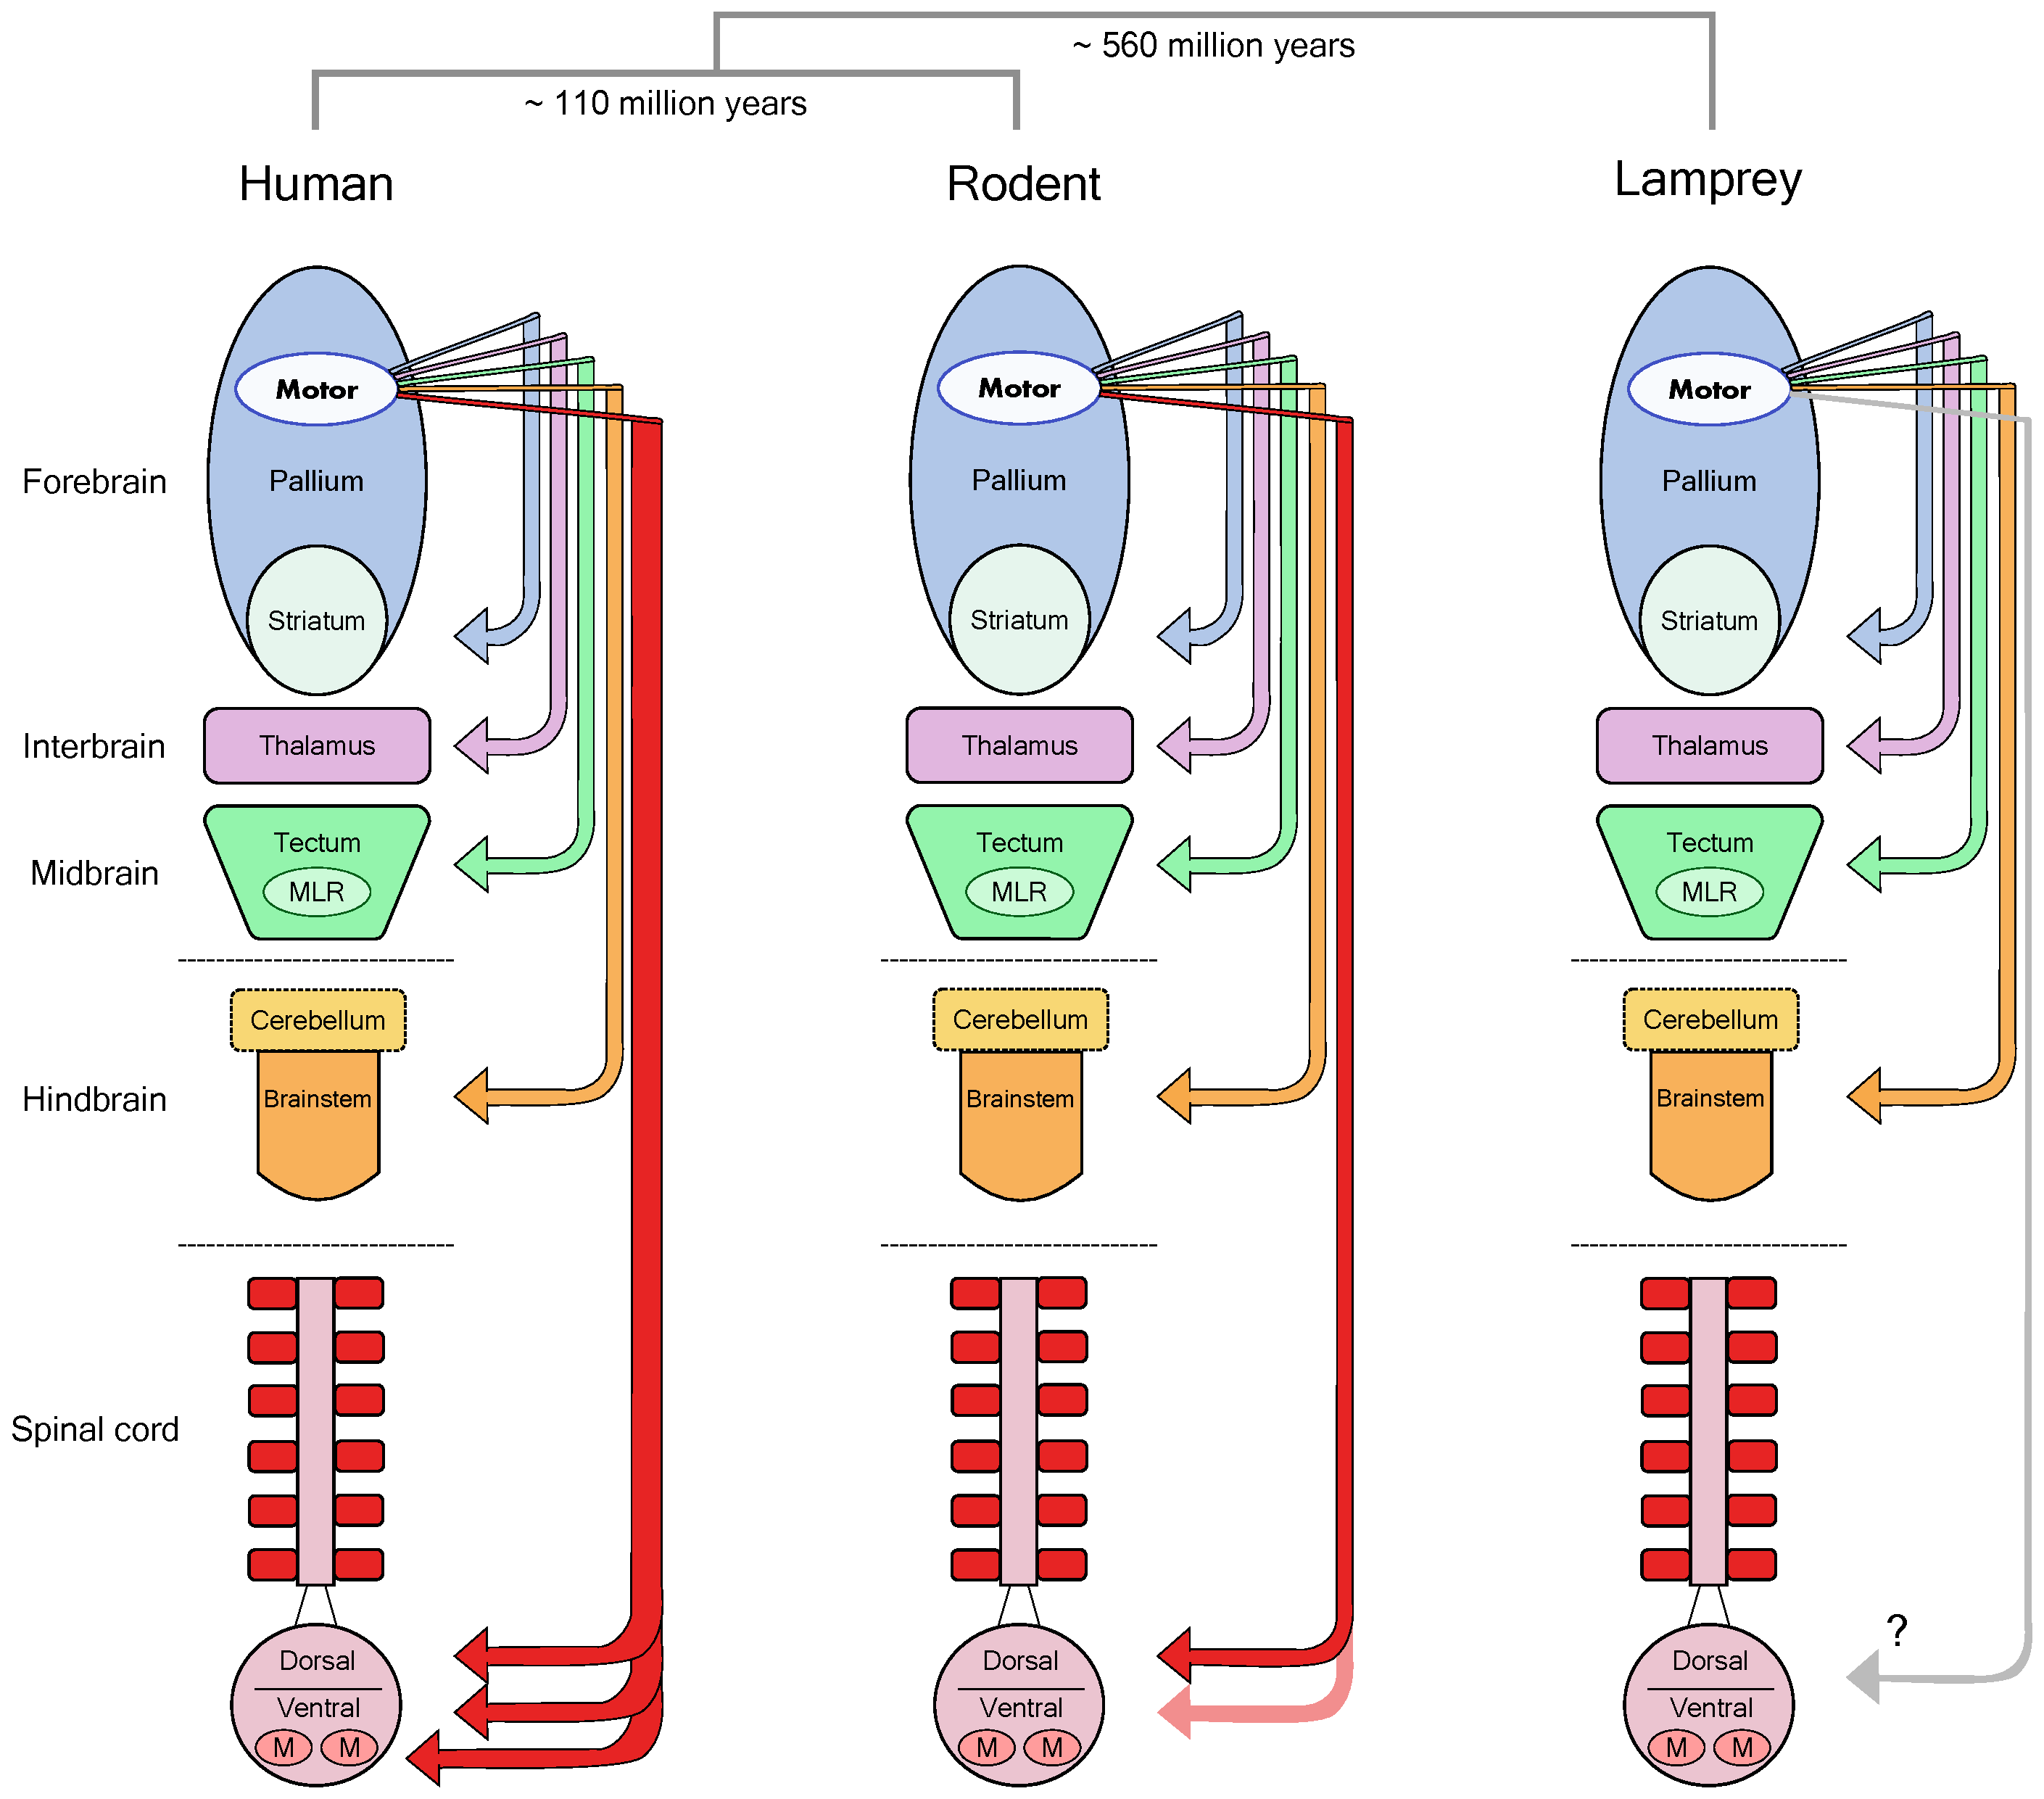
\includegraphics[width=\columnwidth]{chapters/figuresChTeleology/descendingTaxa}
\end{center}
\vspace{-5mm}
\caption{Forebrain motor control pathways across different vertebrate taxa. The molecular divergence times between human (primate), rodent and lamprey groups \protect\cite{Kumar1998} are noted above a schematic view of the major divisions in the vertebrate brain. Arrows indicate the descending monosynaptic projections identified in each group from motor regions of the forebrain pallium to lower motor centres. Note the specialized monosynaptic projection directly targeting spinal motor neurons in human. MLR, Mesencephalic Locomotor Region; M, Motor Neurons.}
\label{fig:descendingTaxa}
\end{figure}

\subsection{Laminar Cytoarchitecture}

Anatomically, there is a clear histological signature of mammalian motor cortex: the loss of granular layer IV. In the canonical layered arrangement of cortical tissue there is a dense layer of cell bodies known as the granular layer that separates the superficial and deep layers. In primary motor cortex this layer is dramatically reduced, earning it the name of agranular cortex. This loss of granular layer seems to be tightly correlated with expansion of the deep layers, especially layer V.

Functionally, layer IV is thought to be the target of feed-forward projections from lower areas in hierarchical models of cortical organization. This view is based on extrapolation from anatomical studies in primary sensory areas where layer IV receives most of the projections from the thalamus, making it the first layer of the cortex to receive direct sensory input. Conversely, layer V is considered the main source of efferents from cortex to subcortical structures.

\subsection{Descending Projections}

Another anatomical landmark of mammalian motor cortex is the presence of a large number of myelinated fibers that descend monosynaptically to the spinal cord. These form the so-called corticospinal, or pyramidal, tract. There is cross over, or decussation, of the tract at the level of the medulla oblongata, which brings the nerve impulses generated by motor cortex mostly to contralateral spinal cord. There is also a smaller bundle of fibres that descend ipsilaterally.

Apart from these direct projections from motor cortex to the spinal cord, there are also many other privileged routes from motor cortex to movement controlling centers in the brainstem. These are also thought to modulate many behaviours via direct brainstem projections to the spinal cord, such as the rubrospinal, tectospinal, vestibulospinal and reticulospinal tracts.

\subsection{Cortico-cortical Projections}

Despite the predominance of descending projections from motor cortex, in recent years a number of studies have revealed the full extent of direct motor cortical outputs, many of them targeting primary sensory areas.

\subsubsection*{There are anatomical differences in corticospinal projections between primates and other mammals}

In primates, the conspicuous effects of motor cortical lesion can also be induced by sectioning the corticospinal tract, the direct monosynaptic projection that connects motor cortex, and other cortical regions, to the spinal cord \cite{Tower1940,Lawrence1968}. In monkeys, and similarly in humans, this pathway has been found to directly terminate on spinal motor neurons responsible for the control of distal muscles \cite{Leyton1917,Bernhard1954} and is also thought to support the low-current movement responses evoked by electrical stimulation of the cortex, as evidenced by the increased difficulty in obtaining a stimulation response following section at the level of the medulla \cite{Woolsey1972}.

However, the corticospinal tract is by no means the only pathway from cortex to movement (Figure \ref{fig:descendingTaxa}). Motor cortex targets many other brain regions that can themselves generate movement. In fact, this specialized connection from telencephalon to spinal cord appeared only recently in vertebrate evolution \cite{TenDonkelaar2009}, and was further elaborated to include a direct connection from cortex to motor neurons only in some primate species and other highly manipulative mammals such as raccoons \cite{Heffner1983}. In all other mammals, including cats and rats, the termination pattern of the corticospinal tract largely avoids the motor neuron pools in ventral spinal cord and concentrates instead on intermediate zone interneurons and dorsal sensory neurons \cite{Kuypers1981,Yang2003}. Why then is there such a large dependency on this tract for human motor control? One possibility is that the rubrospinal tract---a descending pathway originating in the brainstem and terminating in the intermediate zone---is degenerated in humans compared to other primates and mammals \cite{Nathan1955,Nathan1982}, and is thought to play a role in compensating for the loss of the corticospinal tract in non-human species \cite{Lawrence1968a,Zaaimi2012}.

It thus seems likely that most mammals rely on ``indirect'' pathways to convey cortical motor commands to muscles. These differences in anatomy might explain the lack of conspicuous, lasting movement deficits following motor cortical lesion in non-primates, but leaves behind a significant question: what is the motor cortex actually controlling in all these other mammals?

\subsubsection*{What is the role of motor cortex in non-primate mammals?}

In the rat, a large portion of cortex is considered ``motor'' based on anatomical \cite{Donoghue1982}, stimulation \cite{Donoghue1982,Neafsey1986} and electrophysiological evidence \cite{Hyland1998}. However, the most consistently observed long-term motor control deficit following motor cortical lesion has been an impairment in supination of the wrist and individuation of digits during grasping, which in turn impairs reaching for food pellets through a narrow vertical slit \cite{Whishaw1991,Alaverdashvili2008a}. Despite the fact that activity in rodent motor cortex has been correlated with movements in every part of the body (not just distal limbs) \cite{Hill2011,Erlich2011}, it would appear we are led to conclude that this large high-level motor structure, with dense efferent projections to motor areas in the spinal cord \cite{Kuypers1981}, basal ganglia \cite{Turner2000,Wu2009}, thalamus \cite{Lee2008}, cerebellum \cite{Baker2001} and brainstem \cite{Jarratt1999}, as well as to most primary sensory areas \cite{Petreanu2012,Schneider2014}, evolved simply to facilitate more precise wrist rotations and grasping gestures. Maybe we are missing something. Might there be other problems in movement control that motor cortex is solving, but that we may be overlooking with our current assays?

